% ===========================================================================
% m21_ldt -- Supplementary Materials S1: Nonword reaction times (draft v3.1)
% Statistics verified against refit_option1_output_PCA62.txt (model m_rt).
% Figure S1 must be regenerated from the refit model.
% ===========================================================================

\section*{S1. Nonword Reaction Times}

\subsection*{Method}

Responses had a deadline of 1,000~ms; trials without a response by the deadline were scored as errors. The analysis included the 62 participants of the analysed sample (see Methods). Three nonword items were excluded: one was presented incorrectly (as the string \textit{ime}), and two were existing English words (\textit{boil} and \textit{trueness}) that no participant rejected. These items were also excluded from the ERP averages.

In this sample, 69.4\% of responses to the remaining nonwords were correct (complex: 59.5\%; simple: 79.4\%), and 14.6\% were timeouts (complex: 17.6\%; simple: 11.5\%). Only correct responses were analysed (4,224 trials). No further trimming was applied; correct RTs ranged from 314 to 993~ms.

RTs were log-transformed to reduce positive skew and analysed with a linear mixed-effects model fit with \texttt{lme4} \citep{batesFittingLinearMixedeffects2015}. Fixed effects were Morphological Complexity (simple vs.\ complex; sum coded, simple $= -0.5$, complex $= +0.5$), log base frequency and log family size (both z-scored across trials and entered as continuous predictors), Orthographic Sensitivity, and Language Proficiency. The individual difference dimensions were entered as main effects only, as indices of overall response efficiency; interactions between morphological variables and individual differences were examined in the ERP analyses. The model included random intercepts for participants and for base (the complex and simple nonwords built on the same base shared an intercept; 100 bases), and by-participant random slopes for Complexity:
\[
\log(\mathrm{RT}) \sim \texttt{Cmplx} + \texttt{BF} + \texttt{FS} + \texttt{OS} + \texttt{LP} + (1 + \texttt{Cmplx} \mid \texttt{Subj}) + (1 \mid \texttt{Base}).
\]
The model was fit by restricted maximum likelihood using the BOBYQA optimiser. Fixed effects were tested with Satterthwaite-approximated degrees of freedom \citep{kuznetsovaLmerTestPackageTests2017}. Estimated marginal means and their 95\% confidence intervals also used Satterthwaite degrees of freedom and are reported in milliseconds after back-transformation from the log scale.

\subsection*{Results}

Complex nonwords were rejected more slowly than simple nonwords ($M_{\mathrm{complex}} = 720.4$~ms, 95\% CI $[695.8, 745.9]$; $M_{\mathrm{simple}} = 687.6$~ms, 95\% CI $[664.4, 711.6]$), $\beta = 0.047$, $SE = 0.006$, $t(59.75) = 8.29$, $p < .001$, $\eta^2_p = .53$ (Figure~S1A). Base frequency had an inhibitory effect, $\beta = 0.016$, $SE = 0.005$, $t(97.89) = 2.99$, $p = .004$, $\eta^2_p = .08$: nonwords with higher-frequency bases were rejected more slowly. Family size did not affect response times, $\beta = -0.006$, $SE = 0.005$, $t(96.54) = -1.21$, $p = .23$. Readers higher in Orthographic Sensitivity responded faster overall, $\beta = -0.040$, $SE = 0.018$, $t(57.42) = -2.19$, $p = .032$, $\eta^2_p = .08$, whereas Language Proficiency had no effect, $\beta = -0.004$, $SE = 0.013$, $t(57.95) = -0.30$, $p = .76$. The model explained 4.9\% of the variance through fixed effects ($R^2_{\mathrm{marginal}} = .049$) and 48.5\% overall ($R^2_{\mathrm{conditional}} = .485$).

\begin{figure}[htbp]
	\centering
	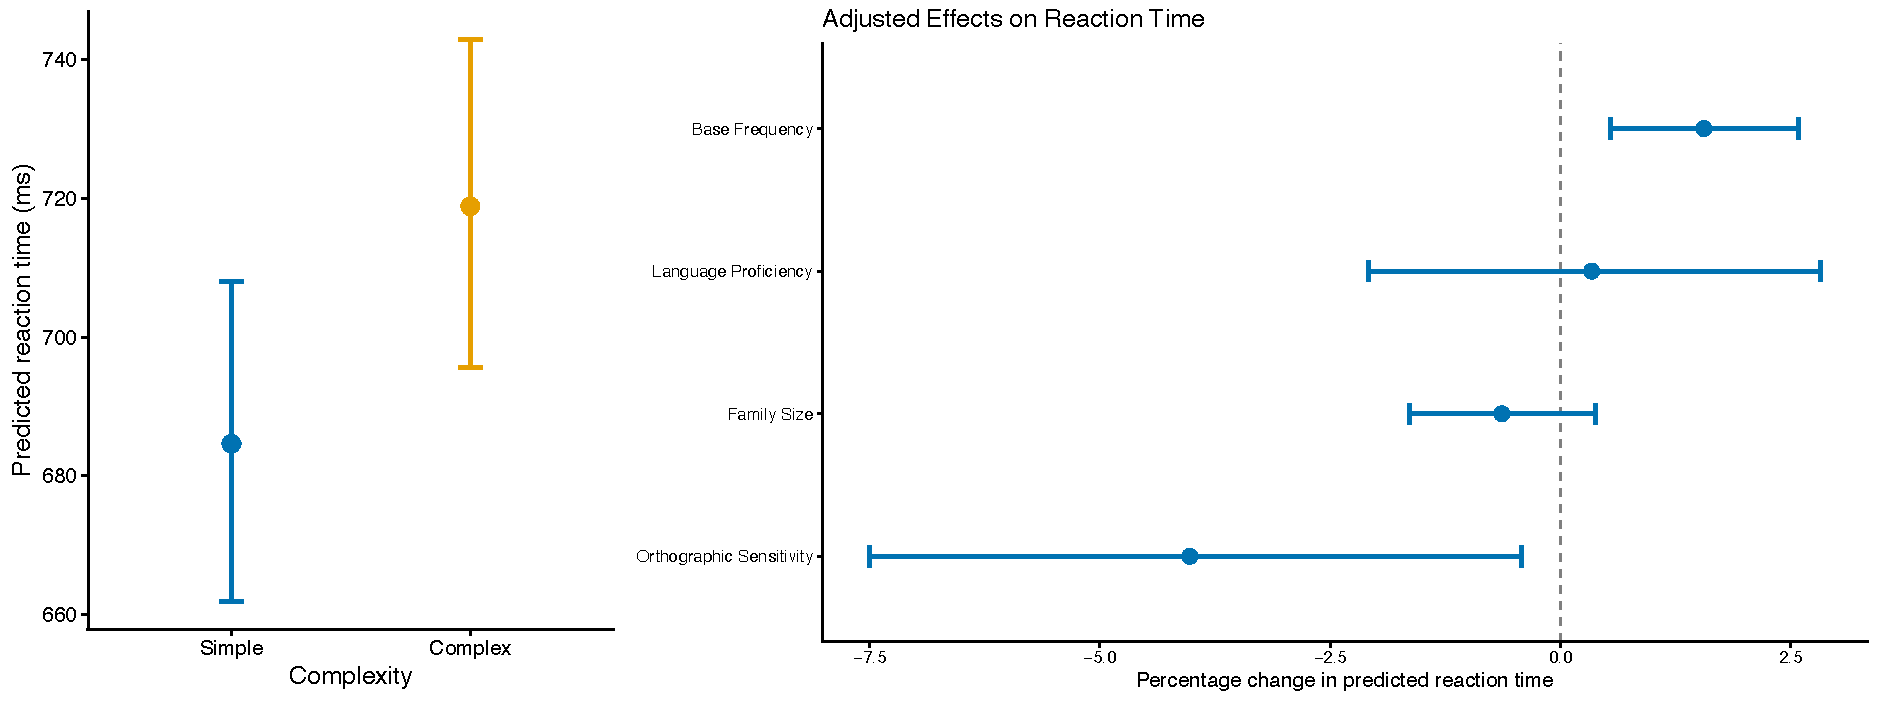
\includegraphics[width=1\textwidth]{Figure 2a NonWords_RT_coefficient_plot} % CHECK: regenerate from the refit RT model.
	\caption*{\textbf{Figure S1.} Nonword reaction time results. (A) Predicted reaction time (ms) by complexity (simple vs.\ complex). (B) Adjusted percentage change in predicted reaction time associated with each predictor (base frequency, family size, Language Proficiency, Orthographic Sensitivity), with 95\% confidence intervals. Complexity and base frequency were associated with significant increases in reaction time and Orthographic Sensitivity with a significant decrease; family size and Language Proficiency were not significant predictors.}
	\label{fig:S1}
\end{figure}
